\section{Appendices}

\textcolor{teal}{\subsection{Brainstorming Ideas}}

\subsubsection{6-3-5 Method} \label{635 method}
\subsubsection*{Hardware \& Mechanics}
\begin{itemize}
    \item use a servo motor for deadbolt control
    \item hall effect sensor to detect if the door is open or closed
    \item implement linear actuator for silent locking
    \item maybe anti-backlash gears to reduce mechanical play
    \item consider designing a modular lock housing with 3D-printed parts
    \item have a backup battery to ensure operation during power outages
\end{itemize}

\subsubsection*{Smartphone Integration}
\begin{itemize}
    \item develop a smartphone app for remote locking/unlocking
    \item push notifications for lock activity (ex: ``Door locked at 3:45 PM'')
    \item have biometric authentication (Face ID or fingerprint)
    \item Use Bluetooth for proximity-based auto-unlock
    \item NFC support for quick unlocking via phone tap
    \item include multi-user access control with time-based permissions
\end{itemize}

\subsubsection*{Security Features}
\begin{itemize}
    \item Implement AES-256 encryption for communication between the lock and phone
    \item maybe two-factor authentication for app access
    \item develop a tamper-detection alarm if the lock is forced
    \item lockdown mode for multiple failed attempts
    \item include a manual override mechanism in case of system failure
    \item utilize rolling codes for Bluetooth pairing to prevent hacking
\end{itemize}

\subsubsection*{Software \& Control}
\begin{itemize}
    \item ESP32 microcontroller for Wi-Fi and Bluetooth control
    \item Develop a closed-loop system to verify if the lock is engaged properly
    \item make a real-time event log accessible via the app
    \item add a scheduling feature for auto-locking at specific times
    \item guest mode with temporary passcodes
    \item Integration with voice assistants like Alexa or Google Assistant
\end{itemize}

\subsubsection*{Advanced Features}
\begin{itemize}
    \item GPS stuff
    \item add geofencing to lock or unlock based on the user's location
    \item integrate with smart home platforms like Home Assistant
    \item use AI-based behavior analysis to suggest locking patterns
    \item add a camera with facial recognition for auto-unlock
    \item enable remote firmware updates
    \item learn database SQL
    \item use solar charging for battery-powered locks
\end{itemize}

% BRAINSTORMING -----------------------------

\subsubsection{Brainstorming} \label{Brainstorming}

\subsubsection*{Adam Wu}
\begin{itemize}
    \item As a person who has amnesia, I would like to be able to find my keys anytime so that when I forget where I place them, I can find them.
    \begin{itemize}
        \item Having a "find my" solution with a key.
    \end{itemize}
    \item As a person who loves security, I would like to have the best lock for my house so that lock pickers are not able to pick my lock.
    \begin{itemize}
        \item Making an “authentication” key that resets the key code within a set time, making it harder for hackers to unlock the door.
    \end{itemize}
    \item As a person who is always last-minute out the door, I fear forgetting to lock the door when I close it.
    \begin{itemize}
        \item Auto-locking door when a person closes the door.
    \end{itemize}
    \item As a person who often forgets to bring their keys, I am scared of getting locked out.
    \begin{itemize}
        \item Having a notification from the key to the phone that alerts: “keys are not close by to you.”
    \end{itemize}
    \item As a parent, I am scared of my kids forgetting their keys and locking themselves out of their room.
    \begin{itemize}
        \item Creating a “master key” that only parents/admins can use to unlock specific doors.
    \end{itemize}
    \item Concerned about key battery life.
    \begin{itemize}
        \item Send a notification to the user when the key is on low battery.
    \end{itemize}
\end{itemize}

\subsubsection*{Nathaniel Laurente}
\begin{itemize}
    \item Key has the ability to notify the user when too far away from the user’s phone/body.
    \item Key deactivates/won’t be able to open the door if too far away from the owner.
    \item “Tap to Pay” technology concept.
    \begin{itemize}
        \item Unlocks the door like a credit card tap on a phone.
        \item If too complex, explore alternative ways to unlock the door.
        \item Eliminates the need for a physical key.
        \item Prevents stolen keys from working if the user still has their phone.
    \end{itemize}
    \item Secure deactivation of the key when too far from the user.
    \begin{itemize}
        \item Possible solution: Use the user's phone for deactivation.
    \end{itemize}
    \item One-time password generator between lock and key to ensure only this exact key can enter the house.
    \item Backup way to get into the house if the user forgets/loses their key.
    \begin{itemize}
        \item Pin access code.
        \item App allows for 2FA authentication using a thumbprint and/or Face ID.
    \end{itemize}
    \item Will the battery last long enough for multiple years?
\end{itemize}

\subsubsection*{Neena Nguyen}
\begin{itemize}
    \item Existing smart lock solutions:
    \begin{itemize}
        \item Smart locks for dorm rooms using mobile apps, passcodes, and scanners.
    \end{itemize}
    \item Who will use this lock?
    \begin{itemize}
        \item People with memory issues (elderly, ADHD).
        \item University students in dorm rooms.
        \item Student ID scanner integration.
        \item Parents with small children (child-proof locks).
    \end{itemize}
    \item Features for parental control.
    \begin{itemize}
        \item Locks after a curfew time.
        \item Prevents children from unlocking without parental approval.
        \item Alerts parents when kids come home from school.
    \end{itemize}
    \item What kind of door lock will it be?
    \begin{itemize}
        \item Facial recognition (requires camera and database knowledge).
        \item Logs entry and exit timestamps.
        \item Digital passcode through an app.
        \item Auto-relocking mechanism after failed attempts.
        \item Bluetooth detection for unlocking within a certain range.
        \item Dual authentication (PIN + scan).
        \item Optional security trigger after specific hours.
        \item Alerts when the door is left unlocked for too long.
        \item Auto-locking after prolonged unlocking.
        \item Detection system to check if the key is on the person.
        \item Prevents intruders from entering without a key.
    \end{itemize}
\end{itemize}

\subsubsection*{Jackson Kennedy}
\begin{itemize}
    \item Normal keys can be lock-picked, but digital keys can be secured based on a communication protocol.
    \item Secure authentication methods.
    \begin{itemize}
        \item PIN authentication with 2FA.
        \item Optimal PIN length (e.g., 4-digit PIN has 1,048,576 combinations).
        \item Brute force prevention strategies.
    \end{itemize}
    \item Preventing communication protocol vulnerabilities.
    \begin{itemize}
        \item What protocol should be used? (Bluetooth has vulnerabilities and short range.)
        \item Cloud-based solutions rely on third-party vendor security.
        \item What information needs to be transferred? (Video data, authentication signals?)
    \end{itemize}
    \item Lock activation logic.
    \begin{itemize}
        \item How exactly will the lock know when to unlock? (Sending a 0 or 1 signal based on specific conditions?)
    \end{itemize}
    \item Security and alerting technologies.
    \begin{itemize}
        \item Sensors to detect nearby people.
        \item Hidden camera or biometric verification for identity confirmation.
    \end{itemize}
    \item Scheduling and timed access.
    \begin{itemize}
        \item Physical locks do not have scheduling options.
        \item Implement timed unlocking (e.g., unlock for 15 minutes for a babysitter).
        \item Extra verification to prevent intruders from exploiting schedules.
    \end{itemize}
\end{itemize}
\newpage

% Begin Morphological Charts ----------------------------------

\subsubsection{Morphological Charts}

\begin{figure}[!ht]
    \centering
    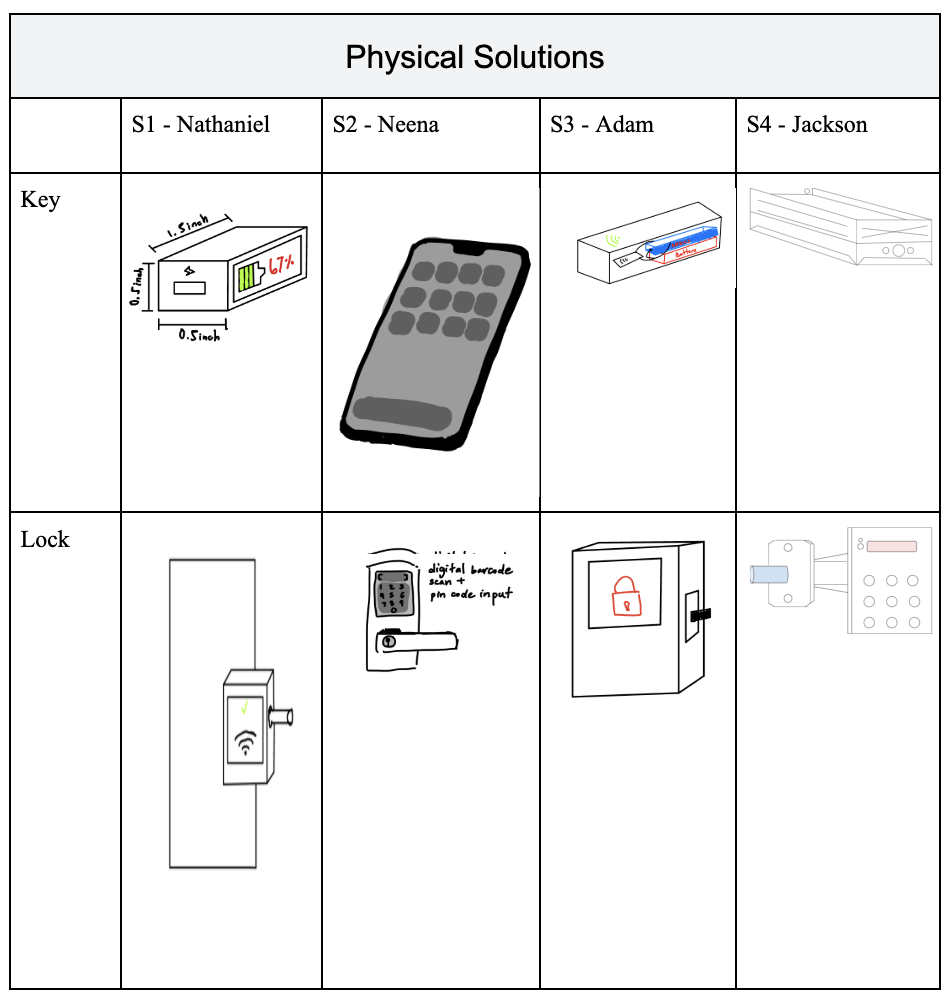
\includegraphics[width=1\linewidth]{./img/p1mm.png}
    \caption{Physical Solution Chart}
    \label{fig:p1mm}
\end{figure}
\newpage
\begin{figure}[!ht]
    \centering
    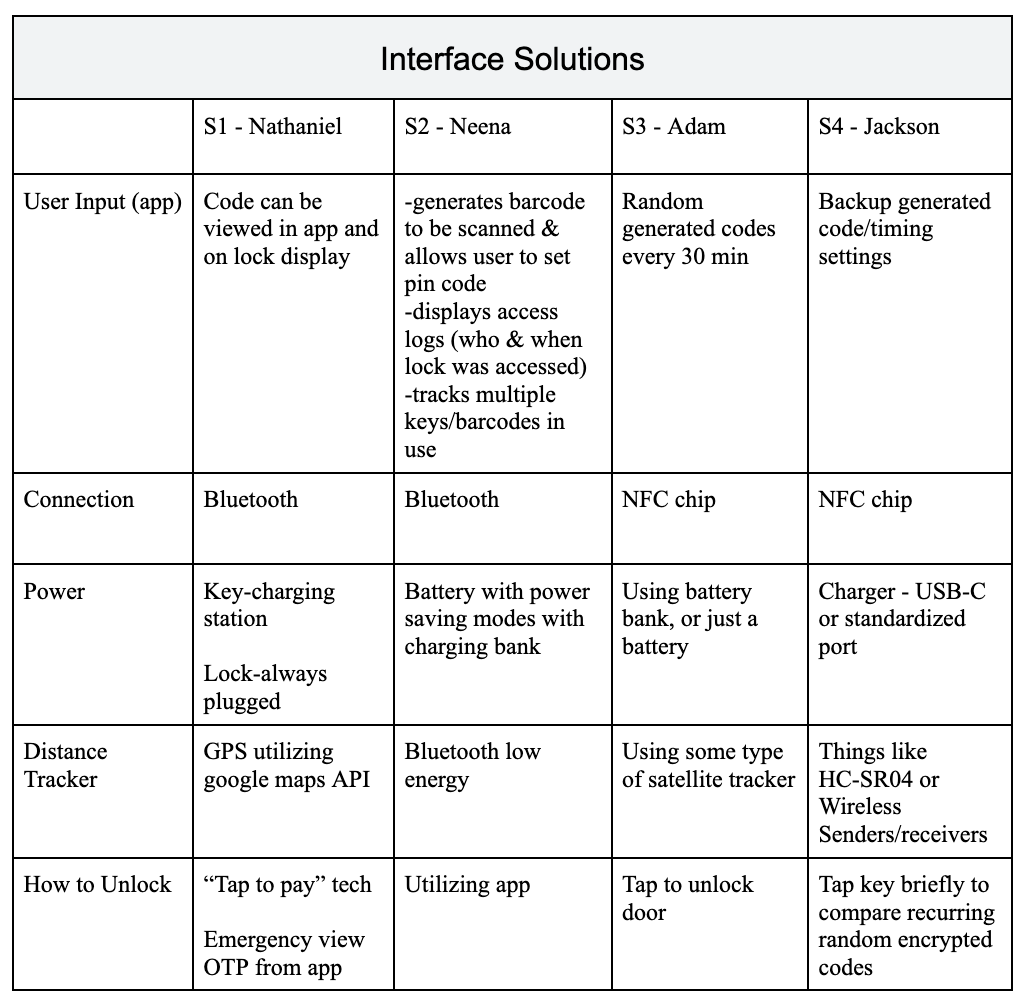
\includegraphics[width=1\linewidth]{./img/p2mm.png}
    \caption{Interface Solutions}
    \label{fig:p2mm}
\end{figure}
\newpage

% Begin Mind Map ---------------------------------------------

\subsubsection{Mind Map}

\begin{figure}[!ht]
    \centering
    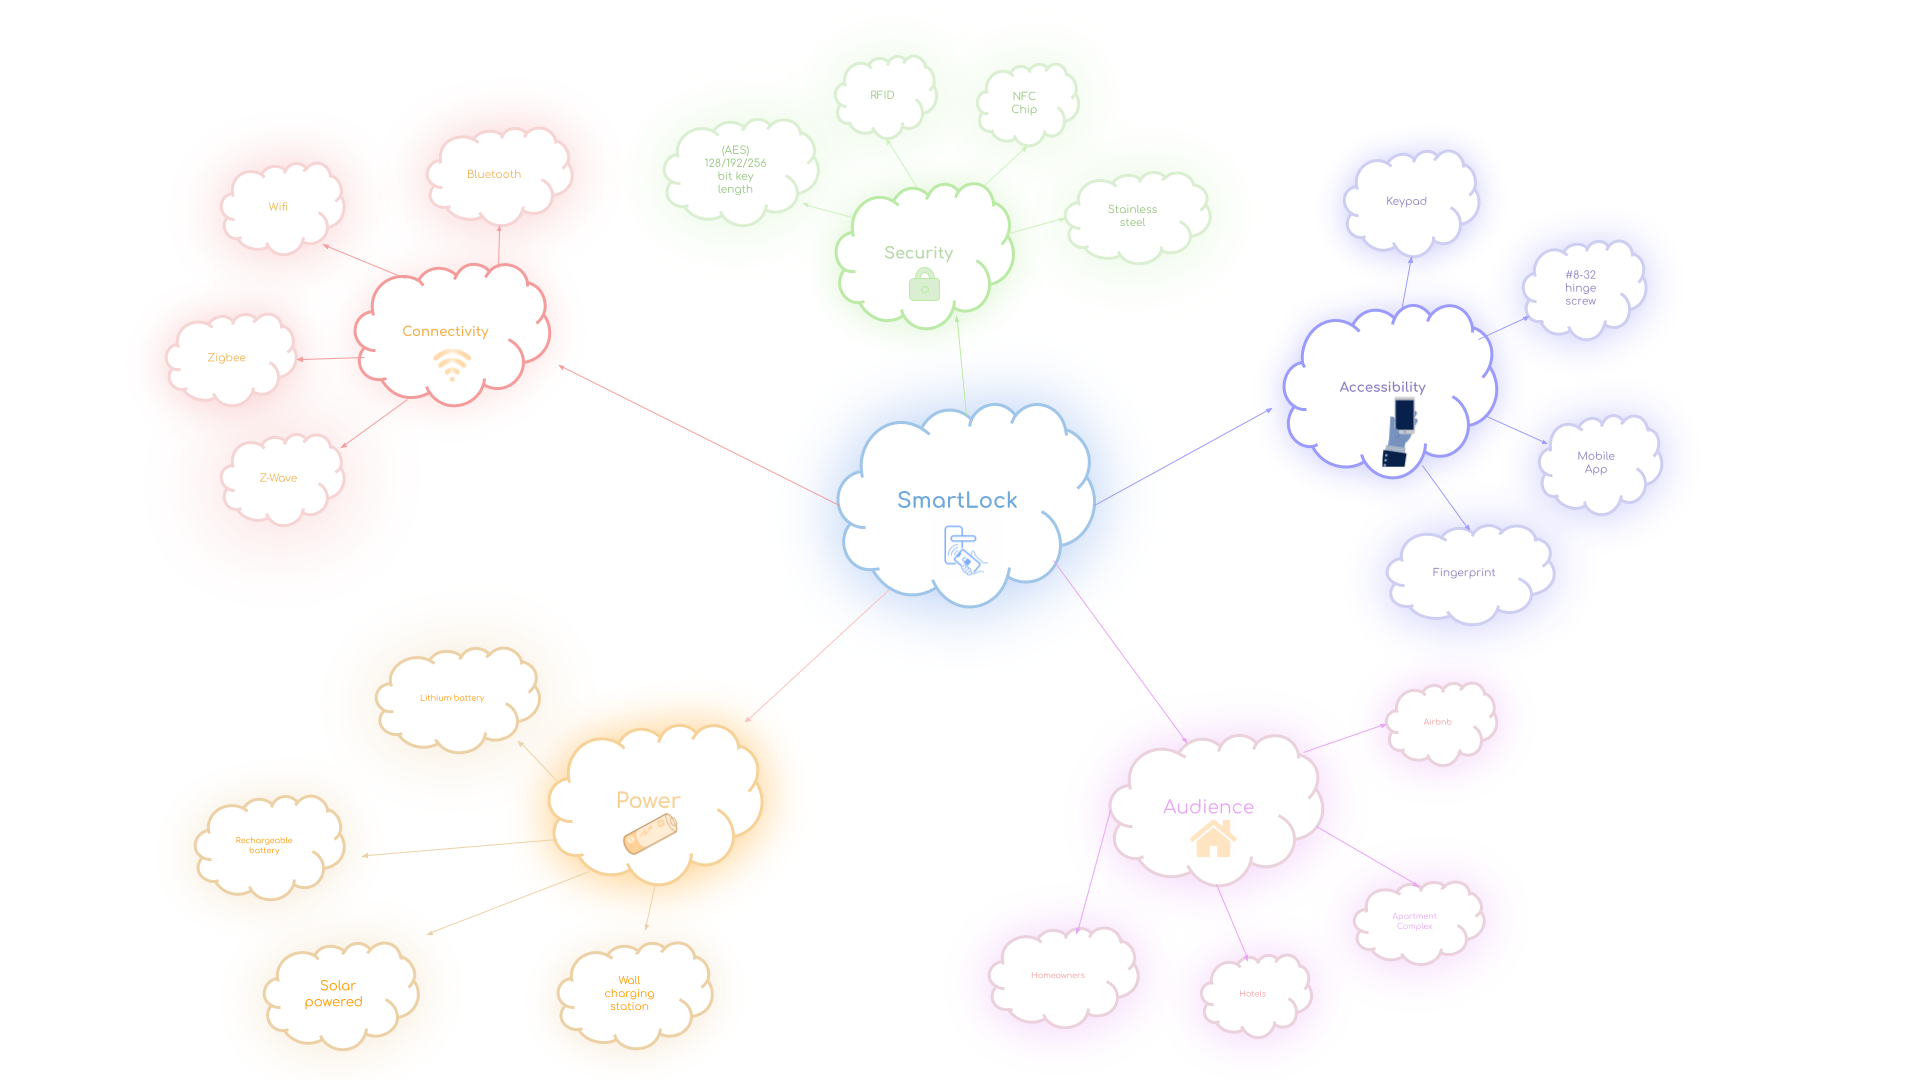
\includegraphics[width=140mm,scale=0.5]{./img/mindmapsmartlock.png}
    \caption{Mind Map}
    \label{fig:mindmapsmartlock}
\end{figure}

\subsubsection{Concept Selection}
\subsubsection*{Weighting Factors}
\begin{tabular}{ll}
    \toprule
    Criteria & Weight (\%) \\
    \midrule
    Security & 40 \\
    Cost & 30 \\
    Power Consumption & 20 \\
    User Convenience & 10 \\
    \textbf{Total} & \textbf{100} \\
    \bottomrule
\end{tabular}

\subsubsection*{Decision Table}
\resizebox{\textwidth}{!}{%
\begin{tabular}{lcccc}
    \toprule
    Criteria & Weight & Design 1 (Basic) & Design 2 (Mid-Range) & Design 3 (Advanced) \\
    \midrule
    Security & 40 & 6 (240) & 8 (320) & 10 (400) \\
    Cost & 30 & 10 (250) & 6 (150) & 3 (75) \\
    Power Consumption & 20 & 6 (90) & 8 (120) & 10 (150) \\
    User Convenience & 10 & 3 (30) & 6 (60) & 9 (90) \\
    \textbf{Total Score} & \textbf{100} & \textbf{680} & \textbf{720} & \textbf{780} \\
    \bottomrule
\end{tabular}%
}

\textbf{Best Design:} Design 3 (Advanced) with 780 points, prioritizing security, cost-efficiency, and power optimization.


\textcolor{teal}{\subsection{Scope}}
\subsubsection*{Firebase Mobile Connectivity Test}
\subparagraph{Test Goals and Purpose}
\begin{itemize}
    \item Ensure that an IOS device can securely connect and push data to the Firebase Firestore servers.
    \item What happens when there may be bad network connection
    \item Set a certain time frame for the pin to be qualified for
\end{itemize}

\subparagraph{Parameters}
\begin{itemize}
    \item 1/0 LOCK$\_$STATE necessary for defining lock-state, 1 is unlocked, 0 is locked.
    \item 7 digit QUALIFIED$\_$PIN list on an allow list for physical keypad on SmartLock.
    \item Make sure what data we send from phone is on firebase
    \item Provide time frame as input for start and expiration time for pin code
\end{itemize}

\subparagraph{Expectations of Test}
\begin{itemize}
    \item There will be no issue with pushing a simple piece of data for LOCK$\_$STATE to the firestore servers, clicking lock will properly push a 0 and clicking unlock will store a 1. Additionally, the pin list composed of generated and custom user pins will also have no trouble being communicated with Firestore servers to later be fetched by the physical device as an additional mechanism for locking and unlocking.
    \item Testing the time frame of the pin code, ensure only the time when valid to use the pin. Otherwise other times should be invalid.
\end{itemize}

\subsubsection{Lock Hardware Functionality Test}
\subparagraph{Test Goals and Purpose}
\begin{itemize}
    \item Ensure that an ESP32-C3 device can securely connect and retrieve data from the Firebase Firestore servers.
    \item Ensure that the ESP32-C3 board can correctly interact with hardware to enable mechanisms for locking/unlocking.
    \item Ensure that invalid codes should not release bolt, while valid codes should.
\end{itemize}


\subparagraph{Parameters}
\begin{itemize}
    \item 1/0 LOCK$\_$STATE necessary for defining lock-state, 0 is locked, 1 is unlocked. Retrieved from firebase.
    \item 7 digit QUALIFIED$\_$PIN list on an allow list for physical keypad on SmartLock.
\end{itemize}

\subparagraph{Expectations of Test}
\begin{itemize}
    \item The locking mechanism will respond appropriately after retrieving from Firestore, and the bolt will trigger when the parameter is set to 0 and likewise release given a 1 value. Additionally, the bolt will release given a valid input from the QUALIFIED$\_$PIN list and reject other non-valid input pins.
    \item Expecting the lock to not unlock after a code is expired, only unlock when it is still valid in a time frame.
\end{itemize}

\subsubsection{Multi-User \& Concurrency Test (Low Priority)}
\subparagraph{Test Goals and Purpose}
\begin{itemize}
    \item Ensure that multiple users can simultaneously interact with the smart lock through the mobile app and keypad without causing system conflicts.
    \item Verify that Firebase can handle concurrent updates to the lock state and PIN list without failure.
    \item Ensure the lock responds appropriately when multiple unlock requests are received from different users.
\end{itemize}


\subparagraph{Parameters}
\begin{itemize}
    \item Simultaneous requests from different mobile devices attempting to unlock/lock the door.
    \item Simultaneous PIN entries from different users on the physical keypad and mobile app.
\end{itemize}

\subparagraph{Expectations of Test}
\begin{itemize}
    \item Multiple users attempting to unlock the door at the same time should not cause conflicts or undefined behavior.
    \item The lock should process and execute the most recent valid request, ensuring no delays or duplicate actions.
    \item System logs should correctly track each user’s request, ensuring accountability and reliable data collection for user feedback.
\end{itemize}
\newpage

% New Section ----------------------------------------------------------------------------------------
\textcolor{teal}{\subsection*{Administrative Details}}

\subsubsection{Firebase Mobile Connectivity Test}
\textbf{\textit{Date $\&$ Location:}} Mar 12, 2025 in class
\newline
\textbf{\textit{Conducting Test:}} Jackson Kennedy, Adam Wu, Nathaniel Laurente, Neena Nguyen, and Professor Harrison.

\subsubsection{Lock Hardware Functionality Test}
\textbf{\textit{Date $\&$ Location:}} Mar 31, 2025 in class
\newline
\textbf{\textit{Conducting Test:}} Jackson Kennedy, Adam Wu, Nathaniel Laurente, Neena Nguyen, and Professor Harrison.

\subsubsection{Multi-User \& Concurrency Test}
\textbf{\textit{Date $\&$ Location:}} April 18, 2025 in class
\newline
\textbf{\textit{Conducting Test:}} Jackson Kennedy, Adam Wu, Nathaniel Laurente, Neena Nguyen, and Professor Harrison.

\textcolor{teal}{\subsection*{Design of Experiment}}
\subsubsection{Firebase Mobile Connectivity Test}
\textbf{\textit{Testing method type:}} Functional Testing, does the simple job of sending unlock or lock to firebase server, also sending pins.
\newline
\textbf{\textit{Test apparatus:}} Firebase Cloud service
\newline
\textbf{\textit{Independent Variables:}} Lock Status, Acceptable Pins
\newline
\textbf{\textit{Dependent Variables:}} N/A
\newline
\textbf{\textit{Number of factors:}}
\newline
\textbf{\textit{Sampling Procedures:}} 2 samples of observing Firestore for 1/0 LOCK$\_$STATE. 2 randomly generated PINs and 1 custom-user pin.

\subsubsection{Lock Hardware Functionality Test}
\textbf{\textit{Testing method type:}} When phone sends data for unlock or lock onto firebase, the lock should quickly retrieve information and respond accordingly. The purpose of this is to make sure the lock receives the data fast enough so that people waiting outside the lock does not wait too long for door to unlock. This should also be similar for the pin code case.
\newline
\textbf{\textit{Test apparatus:}} Utilize ESP32-C3 alongside a Solenoid door lock.
\newline
\textbf{\textit{Independent Variables:}} Make sure that the ESP32-C3 can read a simple "Hello world" on the server for basic testing.
\newline
\textbf{\textit{Dependent Variables:}} Everytime we are generating a new code from phone to firebase, the ESP32-C3 should also be able to retrieve those codes as valid codes immediately.
\newline
\textbf{\textit{Number of factors:}} N/A factors considered in this moment
\newline
\textbf{\textit{Sampling Procedures:}} Samples obtained from servers for LOCK\_STATE, only 0 or 1. Then we have samples for pin codes as well from Firebase.
\newline

\subsubsection{Multi-User \& Concurrency Test}
\textbf{\textit{Testing method type:}} Multiple phones will send an unlock signal from phone at nearly the exact same time and see if any undefined behavior occurs. Send a lock signal and an unlock signal at the same time to test if we can prioritize actions that came first, or lock the app after an action from one device has been made.
\newline
\textbf{\textit{Test apparatus:}} Mobile Device along with ESP32-C3.
\newline
\textbf{\textit{Independent Variables:}} Make sure that the ESP32-C3 can read a simple "Hello world" on the server for basic testing.
\newline
\textbf{\textit{Dependent Variables:}} ESP32-C3 behavior after multiple devices send a signal at the same time or immediately one after the other.
\newline
\textbf{\textit{Number of factors:}} 2 factors to be considered
\newline
\textbf{\textit{Sampling Procedures:}} Samples obtained from servers for LOCK\_STATE, only 0 or 1. Determine if multiple signals causes undefined or expected behavior.



\textcolor{teal}{\subsection*{Testing Procedures}}
\subsubsection{Safety Precautions}
Safety precautions for our project includes not having fast and forceful locks that can hurt individuals.

\subsubsection{Data Collection Method}
Collect data from the phone providing the custom pins onto firebase, as well as collecting data for locking or unlocking. We will also note down which users are grouped together to be able to use the same pin for unlcocking door.

\subsubsection{Observation of External Factors}
Some external factors that could make our product not function properly could include:

\begin{itemize}
    \item Bad network connection from phone or from ESP32-C3
    \item Firebase not loading properly
\end{itemize}